\chapter{Neutrino physics}
\section{Neutrinos in the Standard Model of Particle Physics}
\label{sec:nuIntro}
Neutrinos are elementary particles, specifically neutral leptons, that, according to the \ac{SM} of Particle Physics, only interact via weak interactions.  
They were first postulated in 1930 by the Austrian physicist Wolfgang Pauli to describe the continuous energy spectrum of beta decay. 
Since only two particles were detectable, the process seemed to violate energy and spin conservation; therefore, Pauli introduced a third, 
unseen spin-1/2 particle to carry away the missing energy and balance the angular momentum.

They were eventually confirmed experimentally in 1956 by Clyde Cowan and Frederick Reines during an experiment conducted at the Savannah River 
nuclear reactor in South Carolina. 
This experiment exploited inverse beta decay, in which the postulated particle —specifically an electron antineutrino ($\overline{\nu}_e$)— 
interacts with a proton to produce a neutron and a positron, as described by Eq. \ref{eq:inverse_beta_decay}.
\begin{equation}
    \label{eq:inverse_beta_decay}
    \overline{\nu}_e + p \rightarrow n + e^{+}
\end{equation}
In the experimental setup, antineutrinos produced by the reactor fission processes interacted with protons in the water of two target tanks, 
yielding a positron and a neutron. The positron quickly annihilated with an adjacent electron, producing two prompt gamma rays. 
Meanwhile, the neutron was thermalized and subsequently captured by the cadmium nuclei of cadmium chloride (CdCl$_2$) dissolved in the water tanks.
As a consequence of this neutron capture, an additional gamma-ray signal was released. The detection of these three gamma-ray signals 
in delayed coincidence provided an unambiguous signature of the antineutrino interaction, definitively confirming the existence of 
both neutrinos and antineutrinos \cite{cowan1956nudetection}.

Within the framework of the \ac{SM}, neutrinos are described as neutral fermions that do not participate in strong or 
electromagnetic interactions. Consequently, they are either singlets under the gauge symmetry of SU$(3)_\text{C} \times \text{U}(1)_\text{EM}$ ore they are grouped with their corresponding charged leptons ($\ell = e, \mu, \tau$) into \ac{LH} weak isospin doublets.

The SU$(2)_\text{L}$ gauge invariance strictly dictates the form of the weak interactions between these active neutrinos and the gauge 
bosons. Said interactions consist of \ac{CC} processes mediated by $W^\pm$ bosons and \ac{NC} ones mediated by the $Z^0$ boson, 
described by the following Lagrangians:
\begin{equation}
    \label{eq:SM-neutrino-lagrangian}
    \begin{aligned}
        \mathcal{L}_\text{CC} &= - \frac{g}{\sqrt{2}} \sum_{\ell} \overline{\nu}_{\text{L},\ell} \gamma^\mu \ell_\text{L}^- W_\mu^+ + \text{h.c.} \\
        \mathcal{L}_\text{NC} &= - \frac{g}{2 \cos \theta_W} \sum_{\ell} \overline{\nu}_{\text{L},\ell} \gamma^\mu \nu_{\text{L},\ell} Z_\mu^0
    \end{aligned}
\end{equation}
where $g$ is the SU$(2)_\text{L}$ coupling constant and $\theta_W$ is the Weinberg weak mixing angle. 

Crucially, the \ac{NC} Lagrangian determines the decay width of the $Z^0$ boson into light, left-handed neutrinos. 
Precision measurements of this invisible decay width at colliders have experimentally constrained the number of active neutrino 
families to three ($N_\nu = 2.9840 \pm 0.0082$ \cite{LEPnumberOFnu}), perfectly matching the three known generations of charged leptons.

% --------------------------------------------------------
% ----------------- FLAVOUR OSCILLATIONS -----------------
% --------------------------------------------------------
\section{Flavour oscillations}

% --------------------------------------------------------
% ---------------- EXPERIMENTAL EVIDENCES ----------------
% --------------------------------------------------------
\subsection[Experimental evidence: the solar neutrinos problem]{Experimental evidence: the solar neutrino problem\footnotemark}
\label{subsec:oscillation-experiments}
\footnotetext{All of what is reported in this paragraph is elaborated from \cite{neutrinosPDG}, unless otherwise specified.}
Electron neutrinos are produced in the Sun in thermonuclear reactions that generate solar energy, namely \ac{pp} chains and \ac{CNO} cycles.

\begin{wrapfigure}{r}{0.6\textwidth}
    \centering
    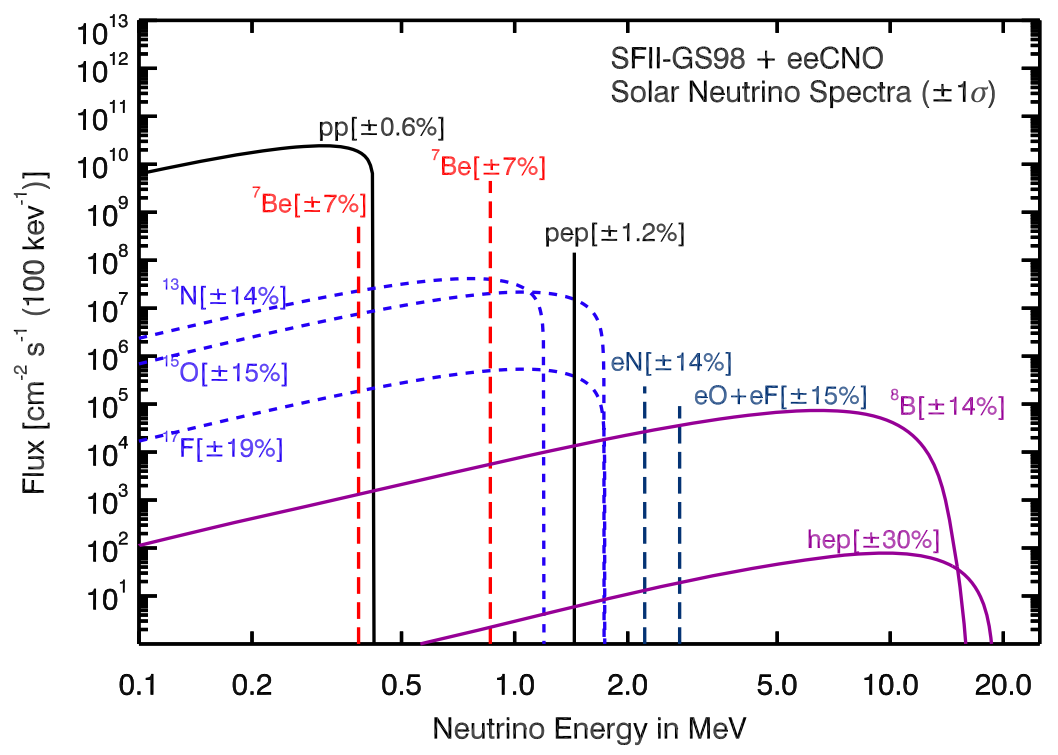
\includegraphics[width=\linewidth]{figures/neutrino-fluxes.png}
    \caption{Energy spectra of solar neutrino fluxes of different reaction processes. Figure taken from \cite{SunNuFluxes}.}
    \label{fig:neutrino-fluxes}
\end{wrapfigure}
In \ac{pp} chains several neutrino-producing reactions are involved, resulting in the overall fusion of four protons into a ${}^{4}$He nucleus ($4p \to {}^4\text{He} + 2e^+ + 2\nu_e$). The total energy released in this reaction is given by the mass difference $Q = 4m_p - m_{{}^4\text{He}} - 2m_e \approx 26 \text{ MeV}$: most of this energy is radiated away by photons, while only a small fraction is carried away by the neutrinos, with an average energy of $\langle E_{2\nu_e} \rangle = 0.59 \text{ MeV}$.

On the other hand, in \ac{CNO} cycles, neutrinos are mainly produced via the decays of ${}^{13}\text{N}$, ${}^{15}\text{O}$ and ${}^{17}\text{F}$. Additionally, electron capture on ${}^{13}\text{N}$, ${}^{15}\text{O}$, and ${}^{17}\text{F}$ produces monoenergetic line spectra of neutrinos, generally referred to as \textit{ecCNO} neutrinos. Compared to the $pp$ chain, \ac{CNO} neutrinos carry away a higher fraction of the reaction energy, with average neutrino energies typically ranging between $0.7\text{ MeV}$ and $1.2\text{ MeV}$. However, the flux of \ac{CNO}-cycle neutrinos is roughly two orders of magnitude lower than the \ac{pp} chains one, accounting for less than $1\%$ of the solar energy production. Therefore it can be neglected in the flux calculation.

Based on the \ac{SSM}, the total expected neutrino flux can be evaluated by considering the total solar luminosity 
($L_{\odot} \approx 3.828 \times 10^{26} \text{ W}$) and dividing it by the net energy released per complete \ac{pp} fusion chain 
($Q \approx 26.73 \text{ MeV}$), while accounting for the spherical propagation of particles across the Earth-Sun distance ($1 \text{ AU}$). 
All these thermonuclear reactions in the Sun exclusively generate electron neutrinos ($\nu_e$) and assuming the absence of neutrino oscillations, 
state-of-the-art calculations predict a theoretical \ac{pp} solar neutrino flux arriving at Earth of approximately 
$\Phi_{\ac{pp}} (\nu_e) \approx 6 \times 10^{10} \text{ cm}^{-2}\text{s}^{-1}$. Figure \ref{fig:neutrino-fluxes} details the fluxes of neutrinos based on the reaction in which they are produced.


\paragraph{The Homestake mine experiment}
The experimental value of the solar neutrino flux $\Phi_{\ac{pp}} (\nu_e)$ has been studied since the last century.
In the late 1960s, the first solar neutrino experiment was performed underground in the Homestake gold mine in South Dakota in order to prevent contaminations of cosmic-ray induced reactions. 
There liquid tetrachloroethylene (C$_2$Cl$_4$) was employed as the target and the \ac{CC} weak interaction $\nu_e + {}^{37}\text{Cl} \longrightarrow e^- + {}^{37}\text{Ar}$ was exploited.
Since this process has an energy threshold of $814$ keV, the fluxes of the ${}^{7}$Be and ${}^{8}$B neutrinos are the most relevant.
Auger electrons from the produced ${}^{37}\text{Ar}$ electron capture were counted to determine the neutrino-chlorine reaction rate.
From the beginning the experimental results yield a neutrino flux of less than one third of what expected, giving birth to the so-called \textit{solar neutrino problem}. 
The final result from the Homestake experiment was $2.56 \pm 0.16 \pm 0.16 \text{ SNU}$~
\footnote{SNU (solar neutrino unit) is a unit of event rate defined as $1 \text{ SNU} = 10^{-36}\text{ captures per second per target atom}$.} \cite{HomestakeResults} 
and can be directly compared with the theoretical \ac{SSM} prediction of $8.46^{+0.87}_{-0.88} \text{ SNU}$~\cite{SSMReference}.

\paragraph{Gallium-based experiments}
Lower-energy components of the solar neutrino spectrum (Figure \ref{fig:neutrino-fluxes}) can be investigated via \ac{CC} interactions exploiting the ${}^{71}\text{Ga}$ process $\nu_e + {}^{71}\text{Ga} \longrightarrow e^- + {}^{71}\text{Ge}$.
Featuring a low energy threshold of $233\text{ keV}$, this reaction is primarily sensitive to \ac{pp} neutrinos, with secondary contributions from ${}^{7}\text{Be}$ sources. 
The produced ${}^{71}\text{Ge}$ nuclei decay via electron capture and allow to measure the capture rate, following an approach analogous to Homestake.
In order to probe this lower-energy regime, two radiochemical experiments were launched at the turn of the 1990s: the SAGE collaboration at the Baksan Neutrino Observatory and the GALLEX (later followed by Gallium Neutrino Observatory (GNO)) experiment at the Laboratori Nazionali del Gran Sasso (LNGS). 
SAGE reported a measured flux of $65.4^{+3.1+2.6}_{-3.0-2.8} \text{ SNU}$, while GALLEX/GNO obtained $69.3 \pm 4.1 \pm 3.6 \text{ SNU}$. 
Both measurements heavily contrast with the \ac{SSM} theoretical prediction of $127.9^{+8.1}_{-8.2} \text{ SNU}$ for the same energy range, reinforcing the solar 
neutrino deficit puzzle.

\paragraph{The Kamiokande experiment} 
Real-time measurements of the solar neutrino flux were pioneered by the Kamiokande experiment and its successor, Super-Kamiokande, located in the Kamioka mine in Japan. 
These water Cherenkov detectors utilized $3000\text{ t}$ of water during the Kamiokande phase in the 1980s, scaling up to $50\text{ kt}$ of ultrapure water for Super-Kamiokande starting in 1996. 
The detectors are sensitive to both \ac{CC} and \ac{NC} interactions, 
which manifest as elastic scattering processes in the form of Eq. \ref{eq:CC-NCwater}.
% , also displayed in Figure \ref{fig:feynman-CCandNCint}.
\begin{equation}
    \label{eq:CC-NCwater}
    \nu_\ell + e^- \longrightarrow \nu_\ell + e^-
\end{equation}
% \begin{figure}[H]
%     \centering
%     \resizebox{0.7\textwidth}{!}{
%         % --- Diagramma 1: Corrente Carica (CC) ---
\begin{tikzpicture}[
    thick,
    fermion/.style={draw=black, postaction={decorate},
        decoration={markings, mark=at position 0.55 with {\arrow{latex}}}},
    boson/.style={draw=black, decorate,
        decoration={snake, amplitude=1.5pt, segment length=5pt}},
    dot/.style={circle, fill=black, minimum size=4pt, inner sep=0pt}
]
    \coordinate (V1) at (0, 1.2);
    \coordinate (V2) at (0, -1.2);
    
    \draw[fermion] (-1.5, 1.8) node[left] {$\nu_e$} -- (V1);
    \draw[fermion] (V1) -- (1.5, 1.8) node[right] {$e^-$};
    \draw[fermion] (-1.5, -1.8) node[left] {$e^-$} -- (V2);
    \draw[fermion] (V2) -- (1.5, -1.8) node[right] {$\nu_e$};
    
    \draw[boson] (V1) -- node[right, xshift=2pt] {$W^+$} (V2);
    
    \node[dot] at (V1) {};
    \node[dot] at (V2) {};
\end{tikzpicture}
\hspace{2.5 cm}
% --- Diagramma 2: Corrente Neutra (NC) ---
\begin{tikzpicture}[
    thick,
    fermion/.style={draw=black, postaction={decorate},
        decoration={markings, mark=at position 0.55 with {\arrow{latex}}}},
    boson/.style={draw=black, decorate,
        decoration={snake, amplitude=1.5pt, segment length=5pt}},
    dot/.style={circle, fill=black, minimum size=4pt, inner sep=0pt}
]
    \coordinate (V3) at (0, 1.2);
    \coordinate (V4) at (0, -1.2);
    
    \draw[fermion] (-1.5, 1.8) node[left] {$\nu_\ell$} -- (V3);
    \draw[fermion] (V3) -- (1.5, 1.8) node[right] {$\nu_\ell$};
    \draw[fermion] (-1.5, -1.8) node[left] {$e^-$} -- (V4);
    \draw[fermion] (V4) -- (1.5, -1.8) node[right] {$e^-$};
    
    \draw[boson] (V3) -- node[right, xshift=2pt] {$Z^0$} (V4);
    
    \node[dot] at (V3) {};
    \node[dot] at (V4) {};
\end{tikzpicture}
%     }
%     \caption{Feynman diagrams of neutrino-electron scatterings. On the left, the \ac{CC} interaction mediated by a $W^+$ boson; on the right, the \ac{NC} 
%     interaction mediated by the $Z^0$ boson. The subscript $\ell$ denotes a generic lepton flavour ($\ell = e, \mu, \tau$).}
%     \label{fig:feynman-CCandNCint}
% \end{figure}

However, the cross-section for $\nu_e$ —the only flavour capable of interacting via the charged current— is approximately six times larger than that for $\nu_\mu$ or $\nu_\tau$. 
Consequently, the elastic scattering signal in standard water is an indistinguishable mixture of \ac{CC} and \ac{NC} events heavily skewed towards $\nu_e$, meaning the detector cannot cleanly measure the total flavor-independent neutrino flux.
Due to energy thresholds of $6.5\text{ MeV}$ in Kamiokande and $3.5\text{ MeV}$ in Super-Kamiokande, these experiments are primarily sensitive to ${}^8\text{B}$ solar neutrinos. The latest results from the Super-Kamiokande collaboration report a measured solar neutrino flux of $(2.345 \pm 0.014 \pm 0.036) \times 10^{6} \text{ cm}^{-2}\text{s}^{-1}$~\cite{latestSUPERK}, exhibiting a strong disagreement with the recent theoretical \ac{SSM} prediction for this energy range, which stands at $(5.46 \pm 0.66) \times 10^{6} \text{ cm}^{-2}\text{s}^{-1}$.

\paragraph{Solution to the solar neutrino problem: the SNO experiment}
The ultimate confirmation of neutrino flavour oscillation arrived with the Sudbury Neutrino Observatory (SNO) experiment that took place in the Creighton Mine near the city of Sudbury (Ontario, Canada) spanning the late 1990s and early 2000s. It exploited $1000\text{ t}$ of heavy water ($\text{D}_2\text{O}$) contained in a spherical acrylic vessel surrounded by a normal water ($\text{H}_2\text{O}$) shield. Unlike Kamiokande, the use of deuterium ($d$) allowed SNO to observe ${}^8\text{B}$ neutrinos not only using the \ac{ES} channel (see Eq. \ref{eq:CC-NCwater}), but also to disentangle the pure \ac{CC} and \ac{NC} interactions detailed in Eq. \ref{eq:deuteron-interactions} and shown in Figure \ref{fig:feynman-deuteron}. 
Importantly, the \ac{CC} interaction on deuterium is sensitive to only $\nu_e$, while the \ac{NC} interaction breaks the deuteron apart and is sensitive to all active flavours of neutrinos with equal cross-sections. 
\begin{equation}
    \label{eq:deuteron-interactions}
    \begin{aligned}
        \nu_e + d &\longrightarrow e^- + p + p \quad (\text{\ac{CC}})\\
        \nu_\ell + d &\longrightarrow \nu_\ell + p + n \quad (\text{\ac{NC}})
    \end{aligned}
\end{equation}
\begin{figure}[H]
    \centering
    \resizebox{0.7\textwidth}{!}{
        % --- Diagramma 1: Corrente Carica (CC) per SNO ---
\begin{tikzpicture}[
    thick,
    fermion/.style={draw=black, postaction={decorate},
        decoration={markings, mark=at position 0.55 with {\arrow{latex}}}},
    boson/.style={draw=black, decorate,
        decoration={snake, amplitude=1.5pt, segment length=5pt}},
    dot/.style={circle, fill=black, minimum size=4pt, inner sep=0pt}
]
    \coordinate (V1) at (0, 1.2);
    \coordinate (V2) at (0, -1.2);
    
    % Linea superiore: neutrino -> elettrone
    \draw[fermion] (-1.5, 1.8) node[left] {$\nu_e$} -- (V1);
    \draw[fermion] (V1) -- (1.5, 1.8) node[right] {$e^-$};
    
    % Linee inferiori: neutrone che diventa protone, e protone spettatore
    \draw[fermion] (-1.5, -1.8) node[left] {$n$} -- (V2);
    \draw[fermion] (V2) -- (1.5, -1.8) node[right] {$p$};
    \draw[fermion] (-1.5, -2.4) node[left] {$p$} -- (1.5, -2.4) node[right] {$p$};
    
    % Bosone scambiato W+
    \draw[boson] (V1) -- node[right, xshift=2pt] {$W^+$} (V2);
    
    \node[dot] at (V1) {};
    \node[dot] at (V2) {};
\end{tikzpicture}
\hspace{2.5 cm}
% --- Diagramma 2: Corrente Neutra (NC) per SNO ---
\begin{tikzpicture}[
    thick,
    fermion/.style={draw=black, postaction={decorate},
        decoration={markings, mark=at position 0.55 with {\arrow{latex}}}},
    boson/.style={draw=black, decorate,
        decoration={snake, amplitude=1.5pt, segment length=5pt}},
    dot/.style={circle, fill=black, minimum size=4pt, inner sep=0pt}
]
    \coordinate (V3) at (0, 1.2);
    \coordinate (V4) at (0, -1.2);
    
    % Linea superiore: neutrino -> elettrone
    \draw[fermion] (-1.5, 1.8) node[left] {$\nu_\ell$} -- (V3);
    \draw[fermion] (V1) -- (1.5, 1.8) node[right] {$\nu_\ell$};
    
    % Linee inferiori: neutrone che diventa protone, e protone spettatore
    \draw[fermion] (-1.5, -1.8) node[left] {$n$} -- (V4);
    \draw[fermion] (V2) -- (1.5, -1.8) node[right] {$n$};
    \draw[fermion] (-1.5, -2.4) node[left] {$p$} -- (1.5, -2.4) node[right] {$p$};

    % Bosone scambiato Z0
    \draw[boson] (V3) -- node[right, xshift=2pt] {$Z^0$} (V4);
    
    \node[dot] at (V3) {};
    \node[dot] at (V4) {};
\end{tikzpicture}
    }
    \caption{Feynman diagrams of neutrino-deuteron scatterings. On the left, the \ac{CC} interaction mediated by a $W^+$ boson; on the right, the \ac{NC} 
    interaction mediated by the $Z^0$ boson. The subscript $\ell$ denotes a generic lepton flavour ($\ell = e, \mu, \tau$).}
    \label{fig:feynman-deuteron}
\end{figure}
The experimental results on solar neutrino fluxes of the ${}^{8}\text{B}$ range are given in Eq. \ref{eq:SNOresults} and taken from \cite{SNO2002-results}:
\begin{equation}
    \label{eq:SNOresults}
    \begin{aligned}
        \Phi_\text{SNO}^\text{CC}(\nu_e) &= (1.76 \pm 0.05 \pm 0.09) \times 10^{6}~\text{cm}^{-2}~\text{s}^{-1} \\
        \Phi_\text{SNO}^\text{ES}(\nu_\ell) &= (2.39 \pm 0.24 \pm 0.12) \times 10^{6}~\text{cm}^{-2}~\text{s}^{-1} \\
        \Phi_\text{SNO}^\text{NC}(\nu_\ell) &= (5.09 \pm 0.44 \pm 0.46) \times 10^{6}~\text{cm}^{-2}~\text{s}^{-1}
    \end{aligned}
\end{equation} 
The total active neutrino flux measured by the \ac{NC} channel, $\Phi_\text{SNO}^\text{NC}(\nu_\ell)$, is remarkably consistent with both the historical \ac{SSM} predictions of that era and the recent updated prediction mentioned above, i.e. $(5.46 \pm 0.66) \times 10^{6} \text{ cm}^{-2}\text{s}^{-1}$. The striking discrepancy between $\Phi_\text{SNO}^\text{NC}(\nu_\ell)$ and the purely electronic $\Phi_\text{SNO}^\text{CC}(\nu_e)$ proved definitively that neutrinos produced in the core of the Sun as purely electron-type are recorded on Earth as a mix of different flavours. 

Finally, this framework also perfectly explains why radiochemical experiments (like Homestake, GALLEX, and SAGE) and water Cherenkov detectors (like Kamiokande and SNO) recorded different deficit ratios: the probability of a neutrino changing flavour is heavily energy-dependent \footnote{See Appendix \ref{app:ThreeFlavoursOscillation}.}. Since these experiments featured different energy thresholds, they probed different ranges of the solar neutrino energy spectrum, naturally observing different survival probabilities.

% ----------------------------------------------------------
% ------------------- VACUUM OCILLATIONS -------------------
% ----------------------------------------------------------

\subsection[Vacuum oscillations]{Vacuum oscillations\footnotemark}
\label{subsec:VacuumOscillations}
\footnotetext{All of what is reported in this paragraph is elaborated from \cite{Thomson}, unless otherwise specified.}
The neutrino flavour transformation confirmed experimentally by Kamiokande and SNO can be explained with the phenomenon of flavour oscillations.
The physical states of particles, i.e. the mass eigenstates, are defined as the stationary states of the free-particle Hamiltonian, 
satisfying Eq. \ref{eq:free-hamiltonian} and following the time evolution of Eq. \ref{eq:time-evolution}.
\begin{equation}
    \label{eq:free-hamiltonian}
    \hat{H} \psi = i \frac{\partial \psi}{\partial t} = E \psi
\end{equation}
\begin{equation}
    \label{eq:time-evolution}
    \psi(\text{\textbf{x}}, \text{t}) = \varphi (\text{\textbf{x}}) e ^{-i \text{Et}}
\end{equation}
The neutrinos mass eigenstates that obey Eq. \ref{eq:free-hamiltonian} and \ref{eq:time-evolution} are labelled $\nu_1$, $\nu_2$ and $\nu_3$ and
there is no reason to believe that such states correspond to the neutrinos weak eigenstates $\nu_e$, $\nu_\mu$ and $\nu_\tau$ that are identified
when the corresponding charged lepton is produced. On the other hand the same basis of mass and weak eigenstates is associated to the charged leptons.


Consider the lepton SU(2)$_\text{L}$ doublet of a given family \textit{i}. This can be written as 
\begin{equation}
    \label{eq:weak-lepton-doublet}
    L_{\text{L}, i} = \begin{pmatrix}
                            \nu_{\text{L}} \\
                            \ell_{\text{L}}
                            \end{pmatrix}_i
\end{equation}
and it is precisely this multiplet that couples to the electroweak gauge bosons in the weak sector of the \ac{SM} Lagrangian written in Eq. \ref{eq:lepton-interaction}.
\begin{equation}
    \label{eq:lepton-interaction}
    \mathcal{L}_{\text{int}} = - \bar{L}_{\text{L}, i} \gamma^\mu \left( g \frac{\tau^a}{2} W_\mu^a + g' Y B_\mu \right) L_{\text{L}, i}
\end{equation}

However when the \ac{SSB} happens and particles acquire mass the terms of the weak doublet can be expressed in terms 
of the new mass eigenstates as written in Eq. \ref{eq:weak-mass-transformation}

\begin{equation}
    \label{eq:weak-mass-transformation}
    \begin{cases}
        \nu_{\text{L}, i} = \text{U}_{\nu \text{L}}~~\nu_{\text{L}, i}^* \\
        \ell_{\text{L}, i} = \text{U}_{\ell \text{L}}~~\ell_{\text{L}, i}^* 
    \end{cases}
\end{equation}

where $\nu_{\text{L}, i}^*$ and $\ell_{\text{L}, i}^*$ are mass eigenstates of a given family \textit{i} for neutrinos and charged leptons respectively.
Consequently current terms undergo the transformation expressed in Eq. \ref{eq:current-masseigen}
\begin{equation}
    \label{eq:current-masseigen}
    \bar{\ell}_{\text{L}, i}~\gamma^{\mu}~\nu_{\text{L}, i} \longrightarrow \bar{\ell}_{\text{L}, i}^*~ U_{\ell \text{L}}^\dagger~\gamma^{\mu}~U_{\nu \text{L}}~\nu_{\text{L}, i}^* = \bar{\ell}_{\text{L}, i}^*~\gamma^{\mu}~\underbrace{U_{\ell \text{L}}^\dagger U_{\nu \text{L}}}_{U_{\text{PMNS}}}~\nu_{\text{L}, i}^* 
\end{equation}
where a new matrix can be highlighted: the Pontecorvo-Maki-Nakagawa-Sakata ($U_\text{PMNS}$) mixing matrix
\footnote{Such rotation matrix is the leptonic equivalent of the Cabibbo-Kobayashi-Maskawa (V$_\text{CKM}$) 
matrix for the quark sector of the SM, with the proper adaptations to be considered.}. 
Named in honor of the physicists who first formulated its theoretical framework \cite{Pontecorvo1957, Pontecorvo1967, Maki1962} 
this matrix establishes a link between the weak (flavour) eigenstates, i.e. $\nu_e$, $\nu_\mu$ and $\nu_\tau$, 
and the stationary (mass) eigenstates, i.e. $\nu_1$, $\nu_2$ and $\nu_3$,
as detailed in Eq. \ref{eq:Upmns}. 
\begin{equation}
    \label{eq:Upmns}
    \begin{pmatrix}
    \nu_e \\
    \nu_\mu \\
    \nu_\tau
    \end{pmatrix}
    =
    \begin{pmatrix}
    U_{e1} & U_{e2} & U_{e3} \\
    U_{\mu1} & U_{\mu2} & U_{\mu3} \\
    U_{\tau1} & U_{\tau2} & U_{\tau3}
    \end{pmatrix}
    \begin{pmatrix}
    \nu_1 \\
    \nu_2 \\
    \nu_3
\end{pmatrix}
\end{equation}

This matrix is a $3 \times 3$ unitary matrix, that parametrises a rotation (a mixing) through some parameters. 
A general $3 \times 3$ matrix can be written in terms of 9 complex numbers, i.e., 18 parameters; 
however, the unitarity property of $U_{\text{PMNS}}$, which means $U U^\dagger = \mathbb{1}$, introduces nine constraints, 
leaving nine independent parameters to fully describe the mixing. Among these nine parameters, three of them are angles, 
$\theta_{12}$, $\theta_{13}$, $\theta_{23}$, while the remaining six are complex phases of the form $e^{i \delta}$ 
since $U_{\text{PMNS}}$ is not a real matrix. Specifically, $\theta_{12}$ is the angle of rotation about the 3-axis, 
$\theta_{13}$ is the angle of rotation about the new 2-axis and $\theta_{23}$ is a rotation about the remaining 1-axis.

Although we have stated above that six complex phases are needed, not all of them carry physical significance. 
In the \ac{SM} framework, the fields of the charged leptons and neutrinos can be redefined multiplying them by arbitrary phase factors. 
Since an overall global phase transformation leaves the physics invariant, exactly five of these six phases can be safely absorbed into 
the definitions of the fermion fields without any observable consequence. Therefore, the $U_{\text{PMNS}}$ matrix is ultimately parametrised 
by only four physical quantities: the three aforementioned mixing angles ($\theta_{12}$, $\theta_{13}$, $\theta_{23}$) and a single, 
irreducible complex phase, $\delta$. This remaining parameter is of fundamental importance, as it is responsible for \ac{CP} violation 
in the lepton sector.

Mathematically, consider that the weak interactions remain invariant under the rephasing of the charged lepton fields
$\ell_\alpha$ (with $\alpha = e, \mu, \tau$) and the neutrino mass eigenstate fields $\nu_k$ (with $k = 1, 2, 3$). 
If we perform the transformations
\begin{equation}
    \ell_\alpha \longrightarrow \ell_\alpha e^{i\theta_\alpha} \qquad \text{and} \qquad \nu_k \longrightarrow \nu_k e^{i\theta_k},
\end{equation}
the elements of the mixing matrix must transform accordingly to leave the Lagrangian unchanged:
\begin{equation}
    U_{\alpha k} \longrightarrow U_{\alpha k} e^{i(\theta_\alpha - \theta_k)}.
\end{equation}
At first glance, it appears we have six independent phases (three from $\theta_\alpha$ and three from $\theta_k$) available to cancel 
the six complex phases of the $3 \times 3$ unitary matrix. However, the transformation depends only on the phase differences. 
If we extract a common overall phase factor, for instance by defining relative phases such that $\theta_\alpha = \theta_e + \theta'_\alpha$ 
and $\theta_k = \theta_e + \theta'_k$, the mixing matrix elements become:
\begin{equation}
    U_{\alpha k} \longrightarrow U_{\alpha k} e^{i(\theta'_\alpha - \theta'_k)}.
\end{equation}
Because the common global phase $\theta_e$ cancels out perfectly, it has no physical effect on the mixing matrix. 
This leaves exactly five independent relative phases ($6$ total fields minus $1$ common phase) that can be strategically chosen to absorb 
five of the original complex phases in $U_{\text{PMNS}}$. The single remaining unabsorbed phase is the Dirac \ac{CP}-violating phase $\delta$.

Finally the full neutrino mixing matrix can be written as reported in Eq. \ref{eq:Upmns-total}
\begin{equation}
    \label{eq:Upmns-total}
    U_{\text{PMNS}} = 
    \begin{pmatrix}
    U_{e1} & U_{e2} & U_{e3} \\
    U_{\mu 1} & U_{\mu 2} & U_{\mu 3} \\
    U_{\tau 1} & U_{\tau 2} & U_{\tau 3}
    \end{pmatrix}
    =
    \begin{pmatrix}
    c_{12}c_{13} & s_{12}c_{13} & s_{13}e^{-i\delta} \\[1ex]
    -s_{12}c_{23} - c_{12}s_{23}s_{13}e^{i\delta} & c_{12}c_{23} - s_{12}s_{23}s_{13}e^{i\delta} & s_{23}c_{13} \\[1ex]
    s_{12}s_{23} - c_{12}c_{23}s_{13}e^{i\delta} & -c_{12}s_{23} - s_{12}c_{23}s_{13}e^{i\delta} & c_{23}c_{13}
    \end{pmatrix}
\end{equation}

or otherwise can be factorised in the product of three different matrices that are detailed in Eq. \ref{eq:Upmns-factorised}
\begin{equation}
    \label{eq:Upmns-factorised}
    U_{\text{PMNS}} = 
    \begin{pmatrix}
    1 & 0 & 0 \\
    0 & c_{23} & s_{23} \\
    0 & -s_{23} & c_{23}
    \end{pmatrix}
    \begin{pmatrix}
    c_{13} & 0 & s_{13}e^{-i\delta} \\
    0 & 1 & 0 \\
    -s_{13}e^{i\delta} & 0 & c_{13}
    \end{pmatrix}
    \begin{pmatrix}
    c_{12} & s_{12} & 0 \\
    -s_{12} & c_{12} & 0 \\
    0 & 0 & 1
    \end{pmatrix}
\end{equation}

where $s_{ij} = \sin(\theta_{ij})$ and $c_{ij} = \cos(\theta_{ij})$.

The reason why we say that are neutrinos to have different flavour and mass eigenstates is that we never directly detect them,
but always their associated charged lepton. In principle instead of Eq. \ref{eq:current-masseigen} we could also write Eq. \ref{eq:current-masseigen-charged}
\begin{equation}
    \label{eq:current-masseigen-charged}
    \bar{\ell}_{\text{L}, i}~\gamma^{\mu}~\nu_{\text{L}, i} \longrightarrow \bar{\ell}_{\text{L}, i}^*~\underbrace{U_{\ell \text{L}}^\dagger U_{\nu \text{L}}}_{U_{\text{PMNS}}}~\gamma^{\mu}~\nu_{\text{L}, i}^* 
\end{equation} 
and consider charged leptons as the oscillating part of the lepton doublet. However since what we detect are indeed charged leptons, these are fixed as both flavour and mass eigenstates while neutrinos flavour states are to be written as a coherent linear superposition of neutrinos mass states through the already mentioned mixing matrix $U_\text{PMNS}$.

A detailed analysis of neutrinos oscillation within three flavours is given in Appendix \ref{app:ThreeFlavoursOscillation}.

%-----------------------------------------------------------
%------------------- MATTER EFFECT -----------------------
%-----------------------------------------------------------

\subsection[Massive neutrinos in matter]{Massive neutrinos in matter\footnotemark}
\footnotetext{All of what is reported in this paragraph is elaborated from \cite{neutrinosPDG}, unless otherwise specified.}
In Paragraph \ref{subsec:oscillation-experiments} we mentioned that the flavour oscillation of solar neutrinos can have two different explanations: they could oscillate in vacuum or they can oscillate directly within the Sun itself through a matter-mediated process known as the \ac{MSW} effect\footnote{The complete quantum mechanical derivation of this effect, starting from the \ac{SM} fermionic currents and phase-space averages, is detailed in Appendix \ref{app:MSW_derivation}.}.

When neutrinos propagate through a dense medium like the solar interior, they interact with the surrounding particles (electrons, protons, and neutrons) via elastic, coherent forward scatterings\footnote{The cross-section of incoherent scatterings is of the order $\sigma \sim \mathcal{O}(10^{-43}\text{cm}^2)$. Therefore, such processes are negligible.}. These coherent interactions macroscopically act as an effective refractive index, which alters the propagation states of the neutrinos.

The fundamental physical asymmetry that drives the \ac{MSW} effect lies in the standard weak interactions. In ordinary matter, all active neutrino flavours ($\nu_e, \nu_\mu, \nu_\tau$) interact with electrons, protons, and neutrons via \ac{NC} interactions mediated by the $Z^0$ boson. Because these interactions are flavour-blind, they induce a common potential for all neutrino flavours. Since neutrino oscillations depend on the \textit{phase differences} between mass eigenstates, this universal \ac{NC} contribution effectively cancels out and does not alter the flavour transition probabilities.

However, ordinary matter is rich in electrons but completely lacks muons and taus. Consequently, only electron neutrinos ($\nu_e$) can undergo Charged Current (\ac{CC}) interactions with the electrons in the medium, mediated by the $W^\pm$ bosons. This exclusive interaction provides an additional potential energy strictly for the $\nu_e$ state, known as the Wolfenstein potential:
\begin{equation}
    % \label{eq:V_C_potential}
    V_C = \sqrt{2} G_F n_e
\end{equation}
where $G_F$ is the Fermi coupling constant and $n_e$ is the electron number density of the medium. For antineutrinos, this potential flips its sign ($V_C = -\sqrt{2} G_F n_e$).

This effective potential modifies the Hamiltonian of the system. As a result, both the mass eigenstates and the mixing angles in matter become dependent on the local electron density $n_e$. For a medium with a continuously varying density gradient, such as the Sun, a neutrino born as a $\nu_e$ in the extremely dense solar core can undergo an adiabatic, resonant transition to another flavour as it travels outwards. This MSW resonance can lead to a near-total flavour conversion even if the vacuum mixing angle is relatively small, elegantly explaining the severe deficit of solar electron neutrinos observed by early experiments on Earth.

%-----------------------------------------------------------
%------------------- NEUTRINO MASSES -----------------------
%-----------------------------------------------------------

\section[Neutrino masses]{Neutrino masses\footnotemark}
\footnotetext{All of what is reported in this paragraph is elaborated from \cite{Thomson}, unless otherwise specified.}
\subsection{\ac{NMO}}
\label{subsec:NMO}
While the complete quantum mechanical derivation of neutrino flavour oscillations is detailed in Appendix \ref{app:ThreeFlavoursOscillation}, it is highly useful to explicitly recall here the final expressions for the transition probabilities. Both the electron neutrino survival probability, $P(\nu_e \to \nu_e)$, and its oscillation probability into other flavours depend heavily on the phase differences between the mass eigenstates during their macroscopic propagation. Evaluating these phase differences in the ultra-relativistic limit reveals that the probabilities are directly governed by the differences of the squared masses of the neutrino stationary states. 

By substituting the kinematic approximations into the expanded probability formula, the electron neutrino survival probability can be explicitly written as:
\begin{equation}
    \label{eq:P_ee_main}
    \begin{aligned}
        P(\nu_e \to \nu_e) = 1 &- 4 |U_{e1}|^2|U_{e2}|^2 \sin^2\left(\frac{\Delta m^2_{21} L}{4E_\nu}\right) \\
        &- 4 |U_{e1}|^2|U_{e3}|^2 \sin^2\left(\frac{\Delta m^2_{31} L}{4E_\nu}\right) \\
        &- 4 |U_{e2}|^2|U_{e3}|^2 \sin^2\left(\frac{\Delta m^2_{32} L}{4E_\nu}\right)
    \end{aligned}
\end{equation}
where $L$ is the oscillation baseline, $E_\nu$ is the neutrino energy, and we introduced the squared mass differences:
\begin{equation}
    \label{eq:mass-differences}
    \begin{aligned}
        \Delta m^2_{21} &= m^2_2 - m^2_1 \\
        \Delta m^2_{31} &= m^2_3 - m^2_1 \\
        \Delta m^2_{32} &= m^2_3 - m^2_2 
    \end{aligned}
\end{equation}

By inspecting Eq. \ref{eq:mass-differences}, it is clear that only two of these differences are independent from one another, while the third can be written as a sum of the other two. Indeed, we can take $\Delta m^2_{21}$ and $\Delta m^2_{32}$ and define $\Delta m^2_{31} = \Delta m^2_{21} + \Delta m^2_{32}$. It is now clear that experimental measurements of neutrino oscillations do not constrain the overall mass scale.

Moreover, to date there are no direct measurements of neutrino masses but only upper limits on them. Specifically we know that
\begin{equation*}
    \sum_{i = 1}^3 m_{\nu_i} \lesssim 1 \text{eV}
\end{equation*}
The most up-to-date experiments reported by the \ac{PDG} \cite{neutrinosPDG} are:
\begin{equation*}
    \begin{aligned}
        \Delta m^2_{21}  &= (7.60 \pm 0.17) \times 10^{-5}~\text{eV}^2 \\
        \Delta m^{2}_{32} &= (2.445 \pm 0.023) \times 10^{-3}~\text{eV}^2 \quad \text{\scriptsize (normal hierarchy)}\\
        \Delta m^{2}_{32} &= (-2.52 \pm 0.04) \times 10^{-3}~\text{eV}^2\quad \text{\scriptsize (inverted hierarchy)}
    \end{aligned}
\end{equation*}
However the absolute mass scale of the neutrinos is not defined and two mass hierarchies are possible as depicted in Figure \ref{fig:mass-ordering}.
\begin{figure}[H]
    \centering
    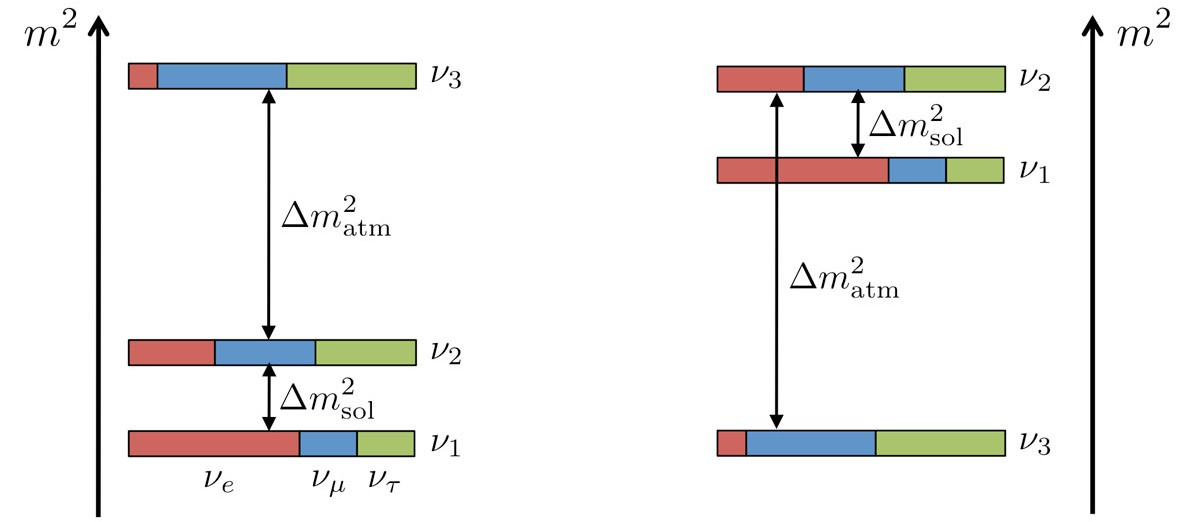
\includegraphics[width = 0.7\textwidth]{figures/mass-hierarchy.jpg}
    \caption{Representation of the two possible mass hierarchies: normal hierarchy on the left and inverted hierarchy on the right. 
    The Figure specifies that $\Delta m^2_{21}$ is obtained via solar neutrinos measurements while $\Delta m^2_{32}$ 
    is given by atmospheric neutrinos experiments. Different colours refer to different neutrino flavours: red for the electron flavour, 
    blue for the muon one and green for the tau, respectively. Figure taken from \cite{fermilab-mass-ordering}.}
    \label{fig:mass-ordering}
\end{figure}


\subsection{The Seesaw mechanism}
\label{subsec:seesaw}
Experimental studies confirm that neutrinos do have masses, therefore there must be a corresponding mass term in the Lagrangian. 
Said term can be introduced in the same way as for the up-type quarks\footnote{Recalling the correspondence u$~\rightarrow~\nu$ and d$~\rightarrow~\ell$ in the SU(2)$_\text{L}$ doublets.} 
using the conjugate Higgs field yielding a Dirac mass term after the \ac{SSB} as expressed in Eq. \ref{eq:neutrinos-dirac-masses}
\begin{equation}
    \label{eq:neutrinos-dirac-masses}
    \mathcal{L}_{D} = - m_D (\overline{\nu}_\text{R}\nu_\text{L} + \overline{\nu}_\text{L}\nu_\text{R}) = -\frac{1}{2}m_D (\overline{\nu_\text{L}}\nu_\text{R} + \overline{\nu_\text{R}^c}\nu_\text{L}^c) + h.c.
\end{equation}
where in the second part we used the equivalence of $\overline{\nu_\text{L}}\nu_\text{R} \longleftrightarrow \overline{\nu_\text{R}^c}\nu_\text{L}^c $.
It is clear that if this is the origin of neutrino masses, then \ac{RH}\footnote{Unless otherwise specified right and left refers to chiral states.}
neutrinos -and \ac{LH} antineutrinos as well- must exist.
However neutrino masses are much smaller than those of other fermions, either the charged leptons or the quarks for which 
masses arise in the Higgs mechanism, suggesting that there might be a different phenomenon to generate neutrino masses.

Seeing that \ac{RH} neutrinos and \ac{LH} antineutrinos transform as singlets in the \ac{SM} transformations, 
any additional term formed by these fields can be added in the the \ac{SM} Lagrangian without breaking its gauge invariance.

While \ac{RH} neutrinos appear as such in the new Lagrangian term, the \ac{LH} antineutrinos are defined as the \ac{CP} conjugate 
fields of \ac{RH} neutrinos as written in Eq. \ref{eq:CPconjugation-righHanded}
\begin{equation}
    \label{eq:CPconjugation-righHanded}
    \psi^c = \hat{C}\hat{P}\psi = i\gamma^2\gamma^0\psi^*.
\end{equation} 
Therefore in the Majorana mass term of Eq. \ref{eq:neutrinos-majorana-masses}, \ac{LH} antineutrinos are written as $\nu_\text{R}^c$ yielding
\begin{equation}
    \label{eq:neutrinos-majorana-masses}
    \mathcal{L}_M = -\frac{1}{2} M \left( \overline{\nu_\text{R}^c} \nu_\text{R} + \overline{\nu_\text{R}} \nu_\text{R}^c \right).
\end{equation}
 

This term clearly respects the local gauge invariance of the \ac{SM}, and consequently it can be added to the \ac{SM} Lagrangian. 
It is now crucial to notice that the Majorana mass term provides a direct coupling between a particle and an antiparticle. 
Thus the corresponding Majorana mass term for the electron would allow $e^+ \leftrightarrow e^-$ transitions, violating charge conservation. 
This problem does not exist for the neutrinos. Nevertheless, seeing that neutrinos are neutral, it is possible that they are their own 
antiparticles, in which case they are referred to as \textit{Majorana neutrinos} and not as \textit{Dirac neutrinos}.

Finally, we can get the general \ac{SM} lagrangian term for neutrino masses including both Eq. \ref{eq:neutrinos-dirac-masses} 
and \ref{eq:neutrinos-majorana-masses} obtaining Eq. \ref{eq:neutrinos-diracANDmajorana-masses}.
\begin{equation}
    \label{eq:neutrinos-diracANDmajorana-masses}
    \mathcal{L}_{DM} = -\frac{1}{2} \left[ m_D \overline{\nu_\text{L}}\nu_\text{R} + m_D \overline{\nu_\text{R}^c}\nu_\text{L}^c + M \overline{\nu_\text{R}^c}\nu_\text{R} \right] + h.c.
\end{equation}
The two different couplings can be represented using Feynman diagrams as depicted in Figure \ref{fig:feynman-massCouplings}.
\begin{figure}[H]
    \centering
    \begin{tikzpicture}[
    thick,
    % Stile per i fermioni (linea continua con freccia a metà)
    fermion/.style={draw=black, postaction={decorate},
        decoration={markings, mark=at position 0.55 with {\arrow{latex}}}},
    % Stile per il campo scalare (linea tratteggiata)
    scalar/.style={draw=black, dashed},
    % Stile per la X
    cross/.style={cross out, draw=black, thick, minimum size=8pt, inner sep=0pt},
    % Stile per il vertice puntiforme
    dot/.style={circle, fill=black, minimum size=4pt, inner sep=0pt}
]

% ---------------- DIAGRAMMA DI DIRAC (Sinistra) ----------------
\coordinate (D) at (0,0);

% Linee entrante e uscente
\draw[fermion] (-1.5, 1.5) node[left] {$\nu_L$} -- (D);
\draw[fermion] (D) -- (1.5, 1.5) node[right] {$\nu_R$};

% Linea tratteggiata (Higgs) con la X finale
\draw[scalar] (D) -- (0, -1.5);
\node[cross] at (0, -1.5) {};

% Vertice centrale con pallino e label
\node[dot, label=right:{$m_D$}] at (D) {};


% ---------------- DIAGRAMMA DI MAJORANA (Destra) ----------------
\coordinate (M) at (6, 0.5); % Spostato a destra e leggermente in alto per allineamento visivo

% Linee (entrambe puntano verso il centro)
\draw[fermion] (4, 0.5) node[left] {$\nu_R$} -- (M);
\draw[fermion] (8, 0.5) node[right] {$\overline{\nu}_L$} -- (M);

% Vertice centrale con la X e label
\node[cross, label=above:{$M$}] at (M) {};

\end{tikzpicture}
    \caption{Feynman diagrams of the two possible mass couplings. On the left the Dirac coupling, associated with $m_D$. On the right the Majorana coupling, associated with $M$.}
    \label{fig:feynman-massCouplings}
\end{figure}

Eq. \ref{eq:neutrinos-diracANDmajorana-masses} can be equivalently rewritten as Eq. \ref{eq:neutrinos-diracANDmajorana-masses-matrix}
\begin{equation}
    \label{eq:neutrinos-diracANDmajorana-masses-matrix}
    \mathcal{L}_{DM} = -\frac{1}{2} \left( \overline{\nu_\text{L}} \quad \overline{\nu_\text{R}^c} \right) \underbrace{\begin{pmatrix} 0 & m_D \\ m_D & M \end{pmatrix}}_{\mathbf{M}} \begin{pmatrix} \nu_\text{L}^c \\ \nu_\text{R} \end{pmatrix} + \text{h.c.}
\end{equation}

where we identified the mass matrix $\mathbf{M}$, that can be diagonalised in order to define the physical states. 
Through the characteristic Eq.$\text{det}(\mathbf{M} - \lambda \mathbb{1})$ that yields $\lambda^2 - M\lambda - m_D^2 = 0$, 
one get the masses of the physical neutrinos that are 
\begin{equation*}
    m_{\pm} = \lambda_{\pm} = \frac{M \pm \sqrt{M^2 + 4m_D^2}}{2} = \frac{M \pm M\sqrt{1 + 4m_D^2/M^2}}{2}.
\end{equation*}
Furthermore, taking the Majorana mass $M$ much greater than the Dirac mass $m$, 
i.e. $M \gg m_D$\footnote{Dirac mass is assumed to be of the same order of the mass of the other fermions ($\mathcal{O}(1~\text{GeV})$) 
while the Majorana mass term is thought to be very large ($\mathcal{O}(10^{11}~\text{GeV})$) in order to get $m_\nu \sim 0.01$~eV}, 
the two possible masses reduce to 
\begin{equation*}
    m_{\pm} \approx \frac{1}{2}M \pm \frac{1}{2}\left( M + \frac{2m_D^2}{M} \right)
\end{equation*}
giving a light neutrino state ($\nu$) and an heavy neutrino state ($N$) with the masses reported in Eq. \ref{eq:final-nu-masses}
\begin{equation}
    \label{eq:final-nu-masses}
    |m_{\nu}| \approx \frac{m_D^2}{M} \quad \text{and} \quad m_N \approx M.
\end{equation} 
Therefore, if we go back to Eq. \ref{eq:neutrinos-diracANDmajorana-masses-matrix} we can rewrite $\nu$ and $N$ as a function of
$\overline{\nu_\text{L}}$, $\overline{\nu_\text{L}^c}$, $\overline{\nu_\text{R}}$ and $\overline{\nu_\text{R}^c}$ as shown in Eq. \ref{eq:neutrinos-revisited}
\begin{equation}
    \label{eq:neutrinos-revisited}
    \nu = \cos\theta (\nu_\text{L} + \nu_\text{L}^c) - \sin\theta (\nu_\text{R} + \nu_\text{R}^c) \quad \text{and} \quad N = \cos\theta (\nu_\text{R} + \nu_\text{R}^c) + \sin\theta (\nu_\text{L} + \nu_\text{L}^c)
\end{equation}
where the mixing angle $\theta$ is determined by the ratio of the Dirac and Majorana masses, with $\theta = \frac{m_D}{M}$. 
Since the Majorana mass scale $M$ is assumed to be enormous compared to the Dirac mass, this ratio is extremely small. 
Consequently, $\theta$ tends to zero and this allows us to apply the small-angle approximations for the trigonometric functions such that
$\tan\theta \sim \theta \sim \frac{m_D}{M}~$ and consequently one gets $~\cos\theta \sim 1~$ and $~\sin\theta \sim \theta = \frac{m_D}{M}~$.\\
This consideration yields
\begin{equation*}
    \nu \approx (\nu_\text{L} + \nu_\text{L}^c) - \frac{m_D}{M}(\nu_\text{R} + \nu_\text{R}^c) ~ \text{and} ~ N \approx (\nu_\text{R} + \nu_\text{R}^c) + \frac{m_D}{M}(\nu_\text{L} + \nu_\text{L}^c).
\end{equation*}
It is now evident that the light-neutrino state is almost entirely \ac{LH} while the heavy-neutrino one is almost entirely \ac{RH}. 
Therefore the latter is not participating in the weak \ac{CC} interactions neither in the weak \ac{NC} interactions of the \ac{SM}.

The process described so far, set against the Higgs mechanism for mass, is known as \textit{seesaw mechanism}.\\
This is just an hypothesis, but it would be more grounded if neutrinos were shown to be Majorana particles.\\
The latter could be done if we would observe the neutrinoless double $\beta$-decay that will be discussed further in this work in Section \ref{subsec:0nubetabeta}.

\section{Beta decay and double beta decay}
Beta decay is a nuclear transition in which a nucleus $(Z, A)$ converts into an isobar $(Z \pm 1, A)$ 
through the weak interaction, with the emission of an electron or positron and the corresponding 
(anti)neutrino, as anticipated in Section~\ref{sec:nuIntro} 
The single-beta-decay process can be written as
\begin{equation}
    \label{eq:single-beta-decay}
    (Z, A) \longrightarrow (Z+1, A) + e^- + \overline{\nu}_e \qquad \text{or} \qquad 
    (Z, A) \longrightarrow (Z-1, A) + e^+ + \nu_e,
\end{equation}
depending on whether a neutron ($\beta^-$) or a proton ($\beta^+$) undergoes the weak transition. 
Enrico Fermi described this process in 1934 by introducing a point-like, four-fermion contact interaction 
Hamiltonian
\begin{equation}
    H_F = G_F \left( \overline{\psi}_p \gamma^\mu \psi_n \right)\left( \overline{\psi}_e \gamma_\mu \psi_\nu \right) + \text{h.c.}
\end{equation} 
with $G_F$ the Fermi coupling constant, later reinterpreted within the \ac{SM} as the low-energy, 
effective limit of the \ac{CC} interaction (Eq. \ref{eq:SM-neutrino-lagrangian}) where a virtual $W$ boson mediates, at the quark level, the $d \to u$ or $u \to d$ transitions. 
The process is allowed whenever it is energetically favourable, i.e. whenever the mass difference between the mother and daughter nuclei is large enough to compensate for the $Q$-value of the reaction, and it is precisely this energy balance, together with nuclear pairing effects, that determines which nuclei undergo ordinary $\beta$ decay and which ones are instead only accessible through the second-order process of double $\beta$ decay, discussed further in this Section.

\subsection{Two-neutrino double beta decay (\texorpdfstring{$2\nu\beta\beta$}{2vbb})}
\label{subsec:2nubetabeta}

Two-neutrino double beta decay ($2\nu\beta\beta$) is a second-order weak interaction process in which a nucleus $(Z, A)$ decays directly into its isobar $(Z+2, A)$ with the simultaneous emission of two electrons and two electron antineutrinos. First proposed in 1935 by Maria Goeppert-Mayer \cite{firstDoubleBeta}, this decay mode perfectly conserves the lepton number and is fully accommodated within the \ac{SM}. The transition is described by the reaction:
\begin{equation}
    \label{eq:2nubetabeta}
    (Z, A) \longrightarrow (Z+2, A) + 2e^- + 2\overline{\nu}_e.
\end{equation}
At the microscopic level, the process occurs through two simultaneous, virtual single-$\beta$ transitions, as illustrated by the two weak vertices in the Feynman diagram in Figure \ref{fig:2nu_feynman}.

\begin{figure}[ht]
    \centering
    \begin{center}
\begin{tikzpicture}[
    thick,
    % Stile per le linee dei fermioni (linea con freccia a metà)
    fermion/.style={draw=black, postaction={decorate},
        decoration={markings, mark=at position 0.55 with {\arrow{latex}}}},
    % Stile per i bosoni W (linea ondulata)
    boson/.style={draw=black, decorate,
        decoration={snake, amplitude=1mm, segment length=3.5mm}},
    % Stile per i vertici dei nucleoni (i cerchi grigi)
    blob/.style={circle, draw=black, fill=gray!30, minimum size=6mm, inner sep=0pt}
]

% ---------------- NUCLEONE SUPERIORE ----------------
% Frecce esterne n e p
\draw[fermion] (-4.5, 2) node[left, font=\Large] {n} -- (-3, 2);
\draw[fermion] (3, 2) -- (4.5, 2) node[right, font=\Large] {p};

% Le 3 linee dei quark all'interno (tra i due blob)
\draw[fermion] (-3, 2.15) -- (3, 2.15);
\draw[fermion] (-3, 2.0) -- (3, 2.0);
\draw[fermion] (-3, 1.85) -- (3, 1.85);

% Bosone W- 
\draw[boson] (0, 1.85) -- (1.5, 0.8);
\node[font=\Large] at (0.4, 1.2) {$W^-$};

% Elettrone e antineutrino 
% (Nota: la linea del neutrino è disegnata da destra a sinistra per invertire la freccia)
\draw[fermion] (1.5, 0.8) -- (3.5, 1.3) node[right, font=\Large] {$e^-$};
\draw[fermion] (3.5, 0.3) node[right, font=\Large] {$\overline{\nu}_e$} -- (1.5, 0.8);


% ---------------- NUCLEONE INFERIORE ----------------
% Frecce esterne n e p
\draw[fermion] (-4.5, -2) node[left, font=\Large] {n} -- (-3, -2);
\draw[fermion] (3, -2) -- (4.5, -2) node[right, font=\Large] {p};

% Le 3 linee dei quark all'interno (tra i due blob)
\draw[fermion] (-3, -1.85) -- (3, -1.85);
\draw[fermion] (-3, -2.0) -- (3, -2.0);
\draw[fermion] (-3, -2.15) -- (3, -2.15);

% Bosone W- 
\draw[boson] (0, -1.85) -- (1.5, -0.8);
\node[font=\Large] at (0.4, -1.2) {$W^-$};

% Elettrone e antineutrino
\draw[fermion] (1.5, -0.8) -- (3.5, -0.3) node[right, font=\Large] {$e^-$};
\draw[fermion] (3.5, -1.3) node[right, font=\Large] {$\overline{\nu}_e$} -- (1.5, -0.8);


% --- DISEGNO I BLOB ---
% (Disegnati per ultimi così coprono perfettamente le estremità delle linee)
\node[blob] at (-3, 2) {};
\node[blob] at (3, 2) {};
\node[blob] at (-3, -2) {};
\node[blob] at (3, -2) {};

\end{tikzpicture}
\end{center}
    \caption{Feynman diagram of $2\nu\beta\beta$. The process proceeds via the exchange of two virtual $W^-$ bosons, resulting in the simultaneous emission of two electrons and two electron antineutrinos.}
    \label{fig:2nu_feynman}
\end{figure}

\begin{wrapfigure}{r}{0.5\textwidth}
    \centering
    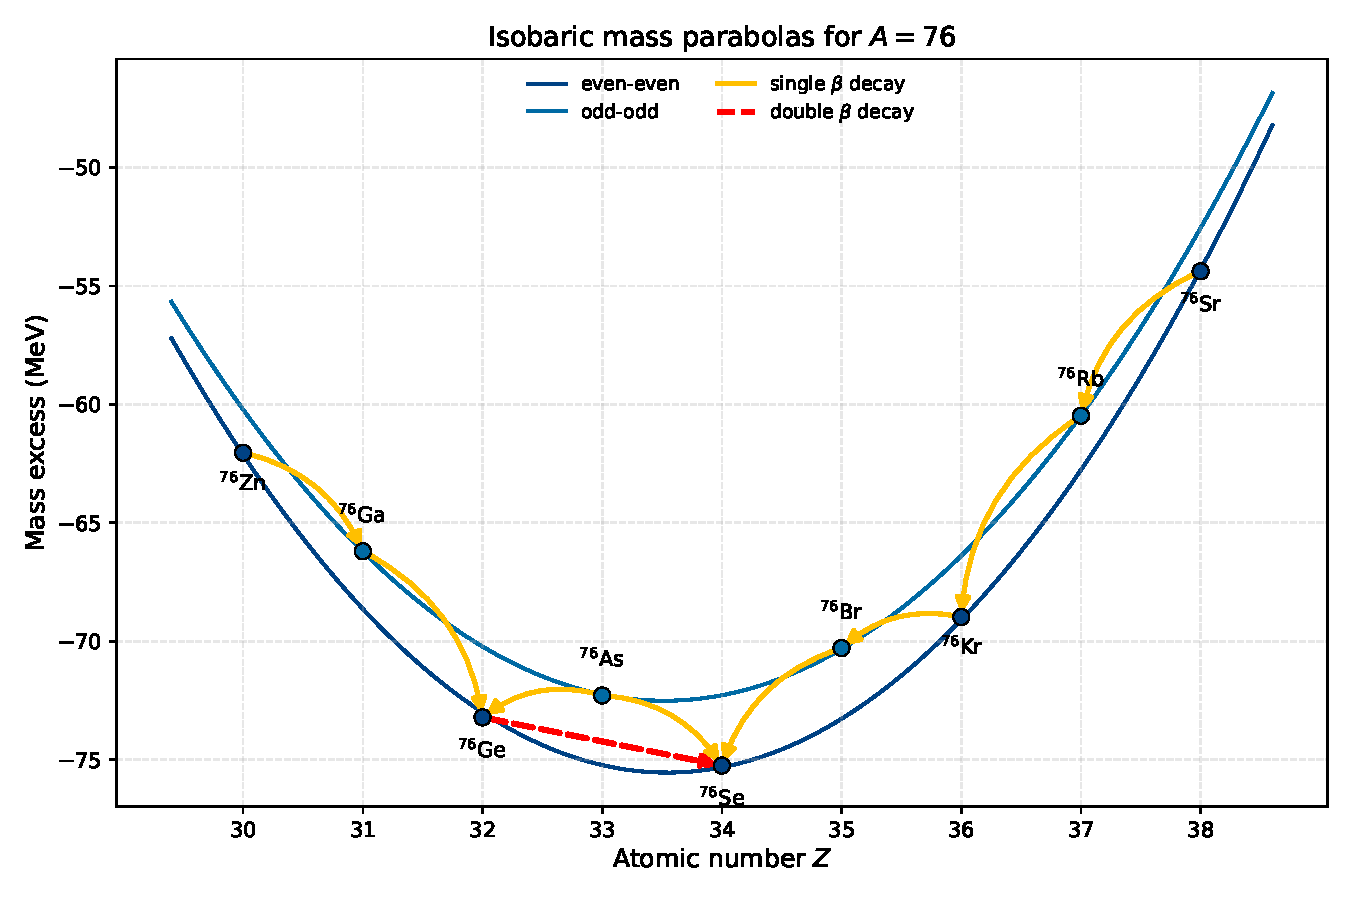
\includegraphics[width=\linewidth]{figures/mass_parabola_A76.pdf}
    \caption{Mass parabola for $A=76$ isobars. A detailed description is given in the text. Custom plot with data taken from \cite{AME2020-masses} and \cite{Ge76-Qvalue}.}
    \label{fig:doublebeta-parabola}
\end{wrapfigure}
For a nucleus to undergo such a rare decay, the standard single-$\beta$ decay to the intermediate isobar $(Z+1, A)$ must be energetically forbidden or heavily suppressed. This kinematic condition naturally arises in even-even nuclei due to the nuclear pairing interaction, which binds them more tightly than their odd-odd neighbours. As a consequence, while the direct transition $(Z, A) \to (Z+1, A)$ is blocked, the target state $(Z+2, A)$ still sits at a lower energy level, effectively opening the double-$\beta$ channel. 
This energy landscape is visualized using mass parabolas, as shown in Figure \ref{fig:doublebeta-parabola} for the case of ${}^{76}\text{Ge}$, where the even-even and odd-odd mass parabolas are shown in dark blue and light blue, respectively. The double-beta transition of ${}^{76}\text{Ge}$ is highlighted in red, while the yellow lines represent ordinary single-$\beta$ decays. The intermediate odd-odd state acts as a virtual state in the quantum mechanical transition and is never physically populated.


Because $2\nu\beta\beta$ is a second-order process in the weak coupling, its decay rate is massively suppressed compared to ordinary $\beta$ decay, resulting in extremely long half-lives of the order of $T_{1/2}^{2\nu} \sim 10^{19}$--$10^{24}$~years, depending on the isotope.

Unlike the neutrinoless mode, $2\nu\beta\beta$ does not require any new physics beyond the \ac{SM} and has been experimentally observed —either directly or via geochemical methods— in about a dozen even-even isotopes. Nuclei such as ${}^{48}\text{Ca}$, ${}^{76}\text{Ge}$, ${}^{82}\text{Se}$, ${}^{100}\text{Mo}$, ${}^{130}\text{Te}$, and ${}^{136}\text{Xe}$ are of particular relevance in modern physics, as they also represent the most promising candidates for the search of the lepton-number-violating neutrinoless double beta decay, which will be extensively detailed in Section \ref{subsec:0nubetabeta}.

\subsection{Neutrinoless double beta decay (\texorpdfstring{$0\nu\beta\beta$}{0vbb})}
\label{subsec:0nubetabeta}

The most sensitive probe to determine whether neutrinos are Dirac or Majorana particles —as introduced in Section \ref{subsec:seesaw}— is the neutrinoless double $\beta$-decay ($0\nu\beta\beta$), detailed in Eq. \ref{eq:0nu-beta-beta} and Figure \ref{fig:0nubetabeta-diagram}:
\begin{equation}
    \label{eq:0nu-beta-beta}
    (Z, A) \longrightarrow (Z+2, A) + 2e^-
\end{equation} 

\begin{figure}[H]
    \centering
    \begin{center}
\begin{tikzpicture}[
    thick,
    % Stile per le linee dei fermioni (linea con freccia a metà)
    fermion/.style={draw=black, postaction={decorate},
        decoration={markings, mark=at position 0.55 with {\arrow{latex}}}},
    % Stile per i bosoni W (linea ondulata)
    boson/.style={draw=black, decorate,
        decoration={snake, amplitude=1mm, segment length=3.5mm}},
    % Stile per la massa di Majorana (la X al centro)
    cross/.style={cross out, draw=black, thick, minimum size=6pt, inner sep=0pt},
    % Stile per i vertici dei nucleoni (i cerchi grigi)
    blob/.style={circle, draw=black, fill=gray!30, minimum size=6mm, inner sep=0pt}
]

% ---------------- NUCLEONE SUPERIORE ----------------
% Frecce esterne n e p
\draw[fermion] (-4, 2) node[left] {n} -- (-2.5, 2);
\draw[fermion] (2.5, 2) -- (4, 2) node[right] {p};

% Le 3 linee dei quark all'interno
\draw[fermion] (-2.5, 2.15) -- (2.5, 2.15);
\draw[fermion] (-2.5, 2.0) -- (2.5, 2.0);
\draw[fermion] (-2.5, 1.85) -- (2.5, 1.85);


% ---------------- NUCLEONE INFERIORE ----------------
% Frecce esterne n e p
\draw[fermion] (-4, -2) node[left] {n} -- (-2.5, -2);
\draw[fermion] (2.5, -2) -- (4, -2) node[right] {p};

% Le 3 linee dei quark all'interno
\draw[fermion] (-2.5, -1.85) -- (2.5, -1.85);
\draw[fermion] (-2.5, -2.0) -- (2.5, -2.0);
\draw[fermion] (-2.5, -2.15) -- (2.5, -2.15);


% --- DISEGNO I BLOB ---
% (Disegnati per ultimi così coprono perfettamente le estremità delle linee)
\node[blob] at (-2.5, 2) {};
\node[blob] at (2.5, 2) {};
\node[blob] at (-2.5, -2) {};
\node[blob] at (2.5, -2) {};


% ---------------- SCAMBIO INTERNO (W, neutrini ed elettroni) ----------------
% Bosoni W (partono dalla linea del quark più vicina al centro)
\draw[boson] (-0.5, 1.85) -- (0.5, 0.7);
\draw[boson] (-0.5, -1.85) -- (0.5, -0.7);

% Linea del neutrino di Majorana (dritta, senza freccia, con la X)
\draw (0.5, 0.7) -- (0.5, -0.7);
\node[cross, label=right:{$\nu_M$}] at (0.5, 0) {};

% Elettroni uscenti
\draw[fermion] (0.5, 0.7) -- (2.5, 1.2) node[right] {e$^-$};
\draw[fermion] (0.5, -0.7) -- (2.5, -1.2) node[right] {e$^-$};

\end{tikzpicture}
\end{center}
    \caption{Feynman diagram for neutrinoless double $\beta$-decay. The Majorana coupling of the neutrino with its own antineutrino (see Figure \ref{fig:feynman-massCouplings}) is shown.}
    \label{fig:0nubetabeta-diagram}
\end{figure}

This hypothetical, lepton-number-violating process can be distinguished from the more common $2\nu\beta\beta$ decay by analyzing the electron energy spectra. Specifically, in $0\nu\beta\beta$ decay, the electrons are produced mono-energetically with a total energy of
\begin{equation*}
    E_e = \frac{1}{2} Q = \frac{1}{2} [M(Z, A) - M(Z+2, A)] 
\end{equation*}
where $M(Z, A)$ and $M(Z+2, A)$ represent the masses of the parent and daughter nuclei, respectively. Conversely, for standard $2\nu\beta\beta$ decay, the combined electron energy spectrum is continuous, with very few events occurring near the endpoint $\frac{1}{2}Q$. This can be visualised in Fig. \ref{fig:Qvalue-2nu0nu}.

\begin{figure}[H]
    \centering
    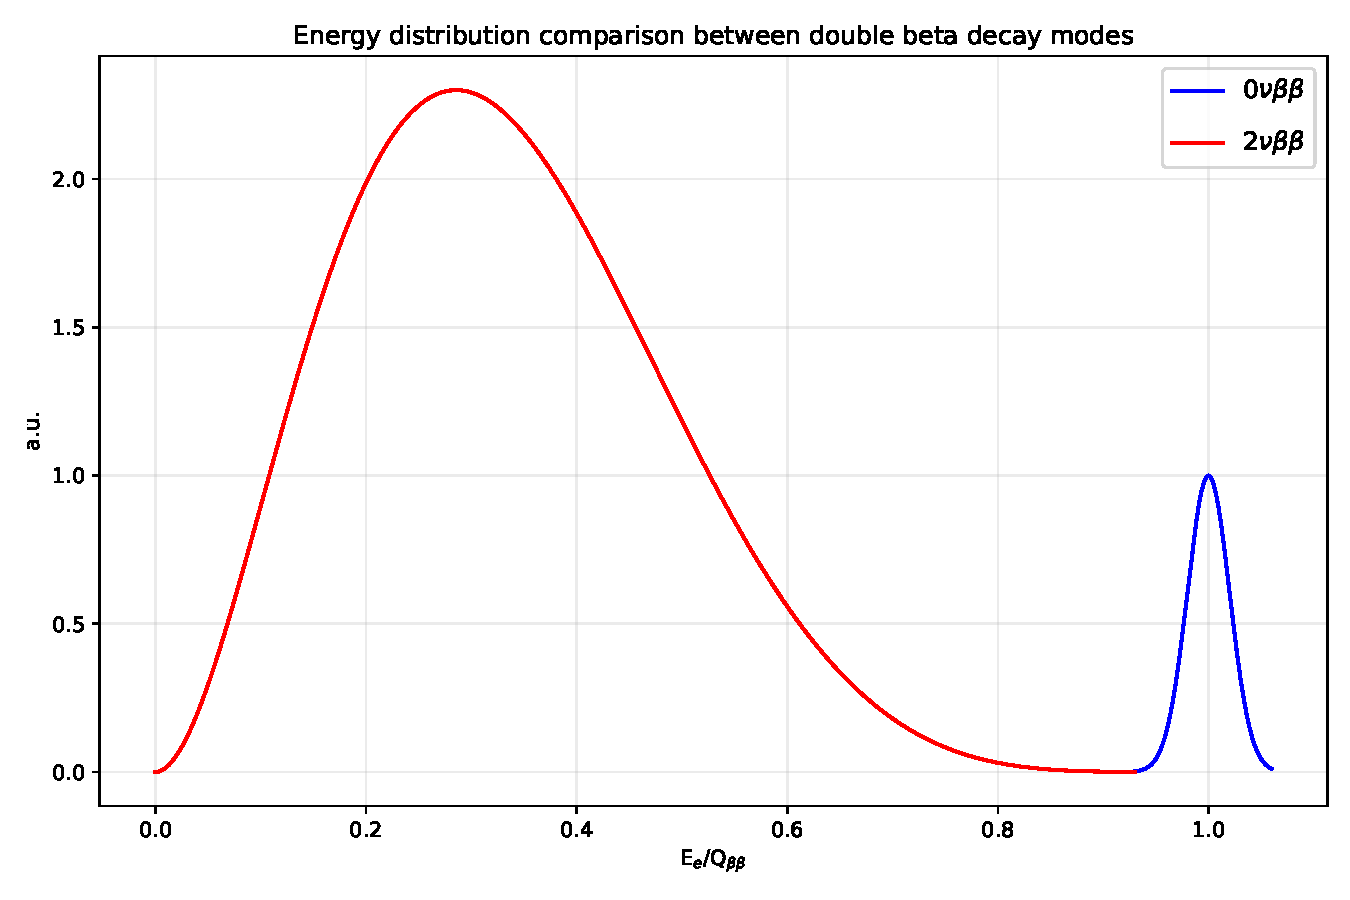
\includegraphics[width=0.6\textwidth]{figures/0nu_vs_2nu.pdf}
    \caption{Schematic representation of the energy distribution for the products in $2\nu\beta\beta$ and $0\nu\beta\beta$ decay modes. The $0\nu\beta\beta$ decay produces a mono-energetic peak at the $Q$-value, while the $2\nu\beta\beta$ decay results in a continuous spectrum.}
    \label{fig:Qvalue-2nu0nu}
\end{figure}

If neutrinos are indeed Majorana particles, the standard mechanism for $0\nu\beta\beta$ decay is mediated by the exchange of a light Majorana neutrino. The decay rate, usually expressed in terms of the half-life $T_{1/2}^{0\nu}$, is given by:
\begin{equation}
    (T_{1/2}^{0\nu})^{-1} = G_{0\nu}(Q, Z) \left| \mathcal{M}_{0\nu} \right|^2 \left( \frac{m_{\beta\beta}}{m_e} \right)^2
\end{equation}
where $G_{0\nu}(Q, Z)$ is the phase space factor (which depends on the Q-value and the atomic number $Z$), $\mathcal{M}_{0\nu}$ is the nuclear matrix element, $m_e$ is the electron mass, and $m_{\beta\beta} = \sum_{i=1}^{3} U_{ei}^2 m_{\nu i}$ denotes the effective Majorana mass, which depends on both the PMNS matrix elements and the neutrino mass eigenvalues. Consequently, the decay rate is directly sensitive to the \ac{NMO}.

From an experimental perspective, observing $0\nu\beta\beta$ decay requires identifying a tiny, mono-energetic signal at $Q_{\beta\beta}$ over the background. For experiments operating in a background-limited regime, the sensitivity to the half-life $S_{1/2}$ scales as:
\begin{equation}
    S_{1/2} \propto \epsilon \cdot a \cdot \sqrt{\frac{M \cdot t}{B \cdot \Delta E}}
\end{equation}
where $\epsilon$ is the detection efficiency, $a$ is the isotopic abundance, $M \cdot t$ is the exposure\footnote{$\text{Exposure [kg yr]} = \text{Detector mass [kg]} \cdot \text{Livetime [yr]}$}, $B$ is the background index (usually expressed in counts/(keV$\cdot$kg$\cdot$yr)), and $\Delta E$ is the energy resolution at $Q_{\beta\beta}$. This formula dictates the design of modern experiments: to maximize sensitivity, one must increase the exposure while minimizing both the background levels and the energy resolution. Specifically, a poor energy resolution causes the continuous tail of the standard $2\nu\beta\beta$ decay to smear into the $0\nu\beta\beta$ region of interest, creating an irreducible background.

To date there are 35 candidate nuclei for neutrinoless double-beta decay, but currently experiments using ${}^{136}$Xe and ${}^{76}$Ge have reported the most sensitive searches for it. However different isotopes needs to be investigated as they offer different uncertainties from
nuclear matrix elements, different backgrounds, and further enable investigation of the mechanism behind the $0\nu\beta\beta$. \cite{neutrinosPDG}

Current experiments investigating this process rely on a variety of detection techniques, most notably liquid scintillators and solid-state semiconductors. For instance, KamLAND-Zen uses a Xenon-loaded liquid scintillator to search for the decay, whereas SNO+ employs a Tellurium-loaded one. In contrast, experiments like LEGEND utilize Germanium semiconductor detectors to probe $0\nu\beta\beta$ processes in ${}^{76}$Ge.

The experimental verification of such an elusive process would constitute a paradigm-shifting milestone in particle physics, laying the cornerstone for physics beyond the \ac{SM} and proving definitively that neutrinos possess an intrinsic nature entirely distinct from all other elementary particles.